% Nier_ANLP -- SemEval-2026 Task 6 (CLARITY) mid-evaluation report.
% Built on the official ACL template (acl-org/acl-style-files @ d5adc82);
% acl.sty and acl_natbib.bst are unmodified copies. Compile with pdfLaTeX + BibTeX.
\documentclass[11pt]{article}

% "final": the camera-ready (non-anonymous) version, as the template's comment describes.
\usepackage[final]{acl}

% Standard package includes (as in the official template)
\usepackage{times}
\usepackage{latexsym}
\usepackage[T1]{fontenc}
\usepackage[utf8]{inputenc}
\usepackage{microtype}
\usepackage{inconsolata}
\usepackage{graphicx}

% Content packages (no layout changes)
\usepackage{amsmath}
\usepackage{amssymb}
\usepackage{booktabs}
\usepackage{xurl}
\usepackage{tikz}
\usetikzlibrary{positioning,arrows.meta,fit,calc,backgrounds}

% Shared notation
\newcommand{\Stwo}{S2}
\newcommand{\Sone}{S1}
\newcommand{\pmsd}[2]{#1\,{\scriptsize$\pm$\,#2}}

% Figures (data figures from clarity/paper_figures.py; the architecture diagram is TikZ)
% Figures. The sections call \FigureArch (text width, sec:intro), \FigureEncSeeds (column width, sec:encoder),
% \FigureLLM (text width, sec:llm) and \FigureExample (column width, sec:analysis).
% The two data-figure PDFs are drawn by clarity/paper_figures.py.

\newcommand{\FigureEncSeeds}{%
\begin{figure}[t]
\centering
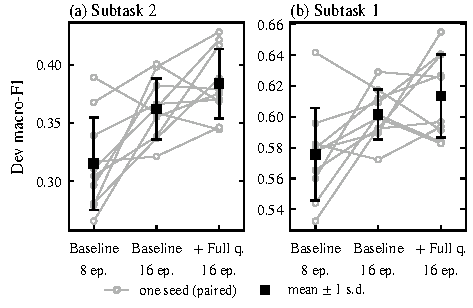
\includegraphics[width=\columnwidth]{figures/fig_deberta_seeds.pdf}
\caption{Single DeBERTa-v3-large models on dev for the three configurations: (a)~\Stwo{} multi-reference macro-F1, (b)~\Sone{} macro-F1. Open circles joined by thin lines are individual seeds, paired across configurations, and filled squares are the mean over the 10 seeds, with error bars of $\pm 1$ standard deviation.}
\label{fig:enc-seeds}
\end{figure}}

\newcommand{\FigureLLM}{%
\begin{figure*}[t]
\centering
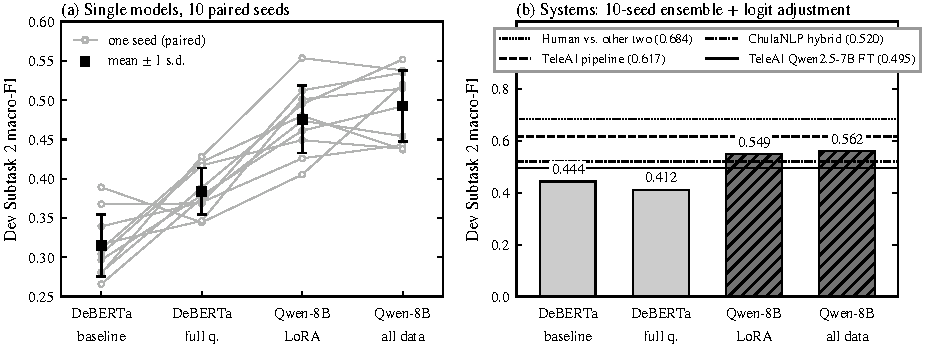
\includegraphics[width=\textwidth]{figures/fig_qwen_vs_deberta.pdf}
\caption{Dev \Stwo{} multi-reference macro-F1 of the DeBERTa-v3-large baseline, DeBERTa with the full question and 16 epochs, Qwen3-8B-Base with LoRA on the same input (3 epochs), and Qwen trained on all of train. (a)~Single models on 10 paired seeds: open circles joined by thin lines are individual seeds, and filled squares are means with $\pm 1$ standard deviation. (b)~The corresponding 10-seed systems (ensemble + logit adjustment, $\tau$ by nested CV, bar height the mean over 10 CV splits), with published dev results as horizontal lines: TeleAI's multi-call pipeline (0.617) and fine-tuned Qwen2.5-7B (0.495) \citep{shi-etal-2026-teleai}, ChulaNLP's DeBERTa top-5 + Kimi-K2 pipeline (0.52) \citep{peerachaidecho-rutherford-2026-chulanlp}, and a human annotator scored against the other two (0.684).}
\label{fig:llm}
\end{figure*}}

\newcommand{\FigureArch}{%
\begin{figure*}[t]
\centering
% Figure 1: the classification pipeline (TikZ, monochrome). Input by \FigureArch in figs.tex.
\begin{tikzpicture}[
  font=\small,
  node distance=2.6mm,
  box/.style={draw, rounded corners=1.5pt, align=center, inner xsep=3pt, inner ysep=3pt, minimum height=#1},
  box/.default=19mm,
  sub/.style={draw, rounded corners=1.5pt, align=center, inner sep=2.5pt, minimum width=#1},
  sub/.default=25mm,
  arr/.style={-{Stealth[length=4pt]}, thin},
  note/.style={font=\footnotesize\itshape, align=center},
  band/.style={draw, densely dotted, rounded corners=2pt, inner sep=2.5pt, align=center, font=\footnotesize},
]
% Input
\node[box, fill=black!6] (in) {%
  \textbf{Input}\\[2pt]
  sub-question $q$\\
  full question $Q$\\
  answer $a$\\[1pt]
  {\footnotesize $\le$ 1{,}024 tokens}};

% Backbone: one of two
\node[sub, right=of in, yshift=5.2mm] (deb) {\textbf{DeBERTa-v3-large}\\{\footnotesize fine-tuned, \texttt{[CLS]}}};
\node[sub, right=of in, yshift=-5.2mm] (qwen) {\textbf{Qwen3-8B-Base}\\{\footnotesize LoRA, last token}};
\node[draw, dashed, rounded corners=2pt, inner sep=2pt, fit=(deb)(qwen)] (bb) {};
\node[note, above=0.3mm of bb] {backbone (one of)};

% Head
\node[box, right=of bb] (head) {\textbf{Linear head}\\[2pt] 9 logits\\ softmax\\[1pt] $p_s(c \mid x)$};

% Seed ensemble: stacked outlines stand for the ten trained seeds
\node[box, right=of head, fill=white] (ens) {\textbf{Mean over}\\\textbf{10 seeds}\\[3pt] $\bar p(c \mid x)$};
\begin{scope}[on background layer]
  \draw[rounded corners=1.5pt, fill=white] ($(ens.south west)+(1.2mm,1.2mm)$) rectangle ($(ens.north east)+(1.2mm,1.2mm)$);
  \draw[rounded corners=1.5pt, fill=white] ($(ens.south west)+(0.6mm,0.6mm)$) rectangle ($(ens.north east)+(0.6mm,0.6mm)$);
\end{scope}

% Logit adjustment
\node[box, right=of ens, xshift=1.2mm] (la) {\textbf{Logit adjustment}\\[2pt]
  $\arg\max\limits_c \dfrac{\bar p(c \mid x)}{\pi_c^{\,\tau}}$};

% Outputs
\node[sub=20mm, fill=black!6, right=of la, yshift=6.6mm] (s2) {\textbf{Subtask 2}\\{\footnotesize evasion type (9)}};
\node[sub=20mm, fill=black!6, right=of la, yshift=-6.6mm] (s1) {\textbf{Subtask 1}\\{\footnotesize clarity level (3)}};

% Arrows
\draw[arr] (in) -- (bb);
\draw[arr] (bb) -- (head);
\draw[arr] (head) -- (ens);
\draw[arr] ($(ens.east)+(1.2mm,0)$) -- (la);
\draw[arr] (la.east) -- ++(1.8mm,0) |- (s2.west);
\draw[arr] (s2) -- (s1);

% Training and decision notes
\path let \p1=(in.west), \p2=(head.east), \p3=(bb.south) in
  node[band, anchor=north, text width=\x2-\x1-5pt] at ({(\x1+\x2)/2}, \y3-2mm) (train) {%
  \textit{Training, per seed:} 3{,}103 train rows, cross-entropy, epoch chosen on the 345-row train slice};
\path let \p1=(ens.west), \p2=(s1.east), \p3=(train.north) in
  node[band, anchor=north, text width=\x2-\x1-5pt] at ({(\x1+\x2)/2}, \y3) (dec) {%
  \textit{Decision:} $\pi_c$ is the class prior on train, and $\tau$ (nested CV) is the only parameter fitted on dev};
\end{tikzpicture}

\caption{The classification system. One backbone (DeBERTa-v3-large, fully fine-tuned, or Qwen3-8B-Base with LoRA) reads the sub-question, the journalist's full question and the answer, and a new linear head gives a distribution over the nine evasion types. A system averages ten seeds and applies logit adjustment, which divides by the train class prior $\pi_c$ raised to $\tau$. The Subtask~1 clarity level follows from the Subtask~2 label through the fixed taxonomy.}
\label{fig:arch}
\end{figure*}}

\newcommand{\FigureExample}{%
\begin{figure}[t]
\centering
\small
\begin{tabular}{@{}p{0.97\columnwidth}@{}}
\toprule
\textbf{Sub-question:} Would you campaign against Senator Joe Lieberman on Iraq? \\
\textbf{Full question:} \ldots{} would you campaign against Senator Joe Lieberman, whose Republican candidate may support you, but he supports you too, on Iraq? \\
\textbf{Answer:} I'm going to stay out of Connecticut. \\
\textbf{Annotators:} Dodging, Dodging, Implicit (\Sone{}: Ambivalent) \\
\bottomrule
\end{tabular}

\medskip
\setlength{\tabcolsep}{4pt}
\begin{tabular}{@{}lll@{}}
\toprule
 & DeBERTa system & Qwen system \\
\midrule
$\bar p$, top 3 & General .373 & Dodging .327 \\
                & Implicit .282 & Implicit .189 \\
                & Deflection .205 & Declining .170 \\
Ensemble argmax & General $\times$ & Dodging $\checkmark$ \\
$\tau$ (item's fold) & 0.70 & 0.85 \\
\Stwo{} after LA & General $\times$ & Declining $\times$ \\
\Sone{} & Ambivalent $\checkmark$ & Clear Non-Reply $\times$ \\
\bottomrule
\end{tabular}
\caption{One dev item through both 10-seed systems ($\checkmark$: in the reference set, or for \Sone{} the gold level). The item was fixed in advance as the error discussed in \S\ref{sec:analysis}. Qwen ranks an acceptable label first, but logit adjustment divides by the train prior (0.205 for Dodging, 0.042 for Declining to answer) and moves the decision to the rarer class.}
\label{fig:example}
\end{figure}}

\newcommand{\FigurePlan}{%
\begin{figure*}[t]
\centering
% Planned system for the final evaluation (TikZ, monochrome, same style as fig_architecture.tex).
% Input by \FigurePlan in figs.tex. Everything in this figure is planned, not run.
% Row 1: input -> M1 -> M2 -> output.  Row 2: M4 (left, under M1) and M3 (right, under M2).
\begin{tikzpicture}[
  font=\footnotesize,
  box/.style={draw, rounded corners=1.5pt, align=center, inner xsep=3pt, inner ysep=3pt},
  plan/.style={box, dashed},
  arr/.style={-{Stealth[length=4pt]}, thin},
  lab/.style={font=\footnotesize, inner sep=1.5pt},
]
% Row 1
\node[box, fill=black!6] (in) {\textbf{Input}\\[1pt] $q$, $Q$, $a$};
\node[plan, right=3.5mm of in] (m1) {\textbf{M1}\enspace Candidate generator\\[1pt]
  {\footnotesize Qwen3-8B + LoRA, $K$ seeds, logit adjustment}\\[1pt]
  {\footnotesize $\bar p(c \mid x)$, candidate set $C(x)$, uncertainty $u(x)$}};
\node[plan, right=5mm of m1] (m2) {\textbf{M2}\enspace Router\\[1pt]
  {\footnotesize defer the fraction $\delta$}\\{\footnotesize with the highest $u(x)$}};
\node[box, fill=black!6, right=18mm of m2] (out) {\textbf{Subtask 2}\\[1pt]{\footnotesize $\rightarrow$ Subtask 1}};

% Row 2
\node[plan, anchor=north west, text width=74mm] (m3) at ($(in.west |- m2.south)+(45mm,-6mm)$) {%
  \centering\textbf{M3}\enspace LLM adjudicator\\[1pt]
  {\footnotesize an open-weight LLM scores only the labels in $C(x)$,
  given definitions, a confusion guide and boundary examples
  retrieved from similar training items, fused with $\bar p$,
  then logit adjustment}};
\node[plan, anchor=north west, text width=36mm] (m4) at (in.west |- m3.north) {%
  \centering\textbf{M4}\enspace Distillation\\[1pt]
  {\footnotesize the adjudicator's decisions on train become
  soft targets for M1, 4-bit inference}};

% Arrows
\draw[arr] (in) -- (m1);
\draw[arr] (m1) -- (m2);
\draw[arr] (m2) -- node[lab, above] {keep, $1-\delta$} (out);
\draw[arr] (m2.south) -- node[lab, right] {defer, $\delta$} (m2.south |- m3.north);
\draw[arr] (m3.east) -| (out.south);
\draw[arr, densely dashed] (m3.west |- m4.east) -- (m4.east);
\draw[arr, densely dashed] (m4.north -| m1.south west) ++(6mm,0) -- ($(m1.south west)+(6mm,0)$);
\end{tikzpicture}

\caption{The planned system for the final evaluation (dashed boxes are new modules, none run yet, see \S\ref{sec:conclusion}). LLM calls per item equal $\delta$, against 1.94 for the winning system \citep{shi-etal-2026-teleai}.}
\label{fig:plan}
\end{figure*}}


\title{HiGrEC: A Controlled Study of Structural Inductive Bias for Response Clarity Classification in Political Interviews}

% Author block as in the team's proposal: names (bold) with roll numbers centred beneath,
% then team and institute. \AND is the template's own command for a new author row.
\author{%
  \begin{tabular}[t]{@{}c@{\hspace{1.1em}}c@{\hspace{1.1em}}c@{\hspace{1.1em}}c@{}}
    Vidvathama R & Siddarth Gottumukkula & Sanjana Reddy Vonteri & Shashikanta Sahoo \\
    {\normalfont\small 2024122002} & {\normalfont\small 2023102040} &
    {\normalfont\small 2026901007} & {\normalfont\small 2026900007}
  \end{tabular}
  \AND
  {\normalfont Team Nier\_ANLP} \\
  {\normalfont International Institute of Information Technology, Hyderabad}}

% PDF document properties (hyperref is loaded by acl.sty; no layout change)
\hypersetup{pdftitle={HiGrEC: A Controlled Study of Structural Inductive Bias for Response Clarity Classification in Political Interviews},
  pdfauthor={Vidvathama R, Siddarth Gottumukkula, Sanjana Reddy Vonteri, Shashikanta Sahoo (Team Nier\_ANLP, IIIT Hyderabad)}}

\begin{document}
\maketitle
\begin{abstract}
SemEval-2026 Task~6 (CLARITY) asks how a politician's answer responds to an interview question.
Subtask~2 has nine evasion types, and each type fixes one of the three clarity levels of Subtask~1.
We set out to find what limits single-pass classifiers on this task, changing one thing at a time and writing down our predictions before every run.
A DeBERTa-v3-large classifier built this way reaches 0.384 multi-reference macro-F1 on Subtask~2 per model, and 0.405 as a ten-seed system with a one-parameter logit adjustment.
Re-ranking, three kinds of hierarchy, rebalanced losses and model soups all failed to improve on it, and the error analysis points at the model rather than at label noise.
When we swap only the backbone for Qwen3-8B fine-tuned with LoRA, keeping the data, input, loss and model selection fixed, Subtask~2 rises by 0.092 and Subtask~1 by 0.095 on every one of ten paired seeds, and the ten-seed system reaches 0.543 and 0.746 (+0.136 on Subtask~2, 95\% CI [0.054, 0.224]).
The gain is spread over most classes instead of sitting on the label boundaries we had expected.
All numbers are on the development set, because the test labels were never released.

\end{abstract}

\section{Introduction}
\label{sec:intro}
\FigureArch

Politicians often answer the question they would have liked to be asked.
\citet{thomas-etal-2024-never} turned this observation into a classification task with a two-level taxonomy of response clarity and evasion, and SemEval-2026 Task~6 \citep{thomas-etal-2026-semeval} made it a shared task.
Subtask~2 asks for one of nine evasion types, and Subtask~1 for one of three clarity levels, which follow directly from the nine types.

The competition was won by pipelines that call a large language model (LLM) several times per item \citep{shi-etal-2026-teleai,peerachaidecho-rutherford-2026-chulanlp}.
Fine-tuned encoders, by contrast, stopped at about 0.50 macro-F1 on Subtask~2 no matter how large they were or how many were ensembled \citep{thomas-etal-2026-semeval}.
A leaderboard cannot tell us \emph{why} the encoders stop there, and the possible reasons predict different things.
If the labels are too noisy to learn, models should fail where annotators disagree.
If the decision rule is wrong for the metric, a better rule should help.
If the model lacks the knowledge needed to read an answer against its question, a larger pretrained model should help under the same protocol.
And if the meaning of the labels cannot be learnt from 3,448 examples, giving the model definitions should help.

We test these explanations with a deliberately controlled single-pass classifier (Figure~\ref{fig:arch}).
Every change is made on its own against a named control, every claim rests on ten paired seeds, our predictions were written down before each run, and nothing is chosen on the development set.
This gives four contributions.
\begin{itemize}
  \item A DeBERTa-v3-large system (\S\ref{sec:encoder}) whose two real improvements, longer training and the full journalist question, are separated from a series of documented failures: re-ranking, hierarchical models, rebalanced losses, per-class thresholds and model soups.
  \item Evidence that the remaining gap lies in the model and not in label noise or the decision rule (\S\ref{sec:analysis}).
  \item A one-change test of the knowledge explanation (\S\ref{sec:llm}). Replacing the backbone with Qwen3-8B-Base fine-tuned with LoRA \citep{qwen3,hu2022lora} improves both subtasks on all ten seeds and lifts the ten-seed system from 0.405 to 0.543 on Subtask~2 and from 0.648 to 0.746 on Subtask~1.
  \item An analysis of where that gain falls, which shows that our own registered prediction was wrong (\S\ref{sec:analysis}).
\end{itemize}
Because the test labels were never released, all comparisons are on the 308-item development set, and we report seed spreads, paired differences and bootstrap intervals throughout.

\section{Problem Statement, Data and Evaluation}
\label{sec:task}

\paragraph{Problem.}
SemEval-2026 Task~6 \citep{thomas-etal-2026-semeval} uses the question--answer pairs of \citet{thomas-etal-2024-never}, taken from U.S.\ presidential interviews.
Each item is a triple $x = (q, Q, a)$.
Here $q$ is a sub-question (median 15 tokens), $Q$ is the journalist's full turn from which it was split (median 62 tokens), and $a$ is the president's entire answer (median 266 tokens).
Let $\mathcal{Y}_9$ be the nine evasion types, $\mathcal{Y}_3$ the three clarity levels, and $g:\mathcal{Y}_9 \rightarrow \mathcal{Y}_3$ the fixed taxonomy map in Table~\ref{tab:taxonomy}.
Subtask~2 (\Stwo{}) asks for $f(x) \in \mathcal{Y}_9$, the way \emph{that particular sub-question} was answered, and Subtask~1 (\Sone{}) asks for a level in $\mathcal{Y}_3$.
Like the top-ranked systems \citep{shi-etal-2026-teleai,peerachaidecho-rutherford-2026-chulanlp}, we learn $f$ and predict $g(f(x))$ for \Sone{}.
We call a classifier \emph{single-pass} if it runs one model once per item, and the question of this paper is what limits such a classifier on this task.

\begin{table}[t]
\centering
\small
\setlength{\tabcolsep}{3.5pt}
\begin{tabular}{@{}llrr@{}}
\toprule
Evasion type & Clarity level & Train \% & Dev sets \\
\midrule
Explicit            & Clear Reply     & 30.5 & 115 \\
\midrule
Implicit            & Ambivalent      & 14.2 & 99 \\
Dodging             & Ambivalent      & 20.5 & 96 \\
General             & Ambivalent      & 11.2 & 113 \\
Deflection          & Ambivalent      & 11.0 & 51 \\
Partial/half-answer & Ambivalent      & 2.3  & 14 \\
\midrule
Declining to answer & Clear Non-Reply & 4.2  & 17 \\
Claims ignorance    & Clear Non-Reply & 3.5  & 15 \\
Clarification       & Clear Non-Reply & 2.7  & 4 \\
\bottomrule
\end{tabular}
\caption{The taxonomy. Each evasion type determines a clarity level. Train \% is the share of the 3,448 training labels, and Dev sets is the number of the 308 dev items whose reference set contains the type.}
\label{tab:taxonomy}
\end{table}

\paragraph{Data.}
The training set has 3,448 items with one label each.
The development (dev) set has 308 items labelled by three annotators, of which 125 are unanimous, 150 split two to one and 33 get three different labels, so the reference set $G_i$ of an item holds one to three types.
The 237 test items have two annotators each, but their labels were never released and the evaluation server has closed, so every comparison in this paper is on dev.
Two properties of the data shaped our modelling.
First, 69\% of training rows share their answer with another sub-question, and 71.7\% of those shared answers carry different labels, so the model has to work out which part of a long answer responds to which sub-question.
Second, the answers are long, and for 101 of the 308 dev items the sub-question and answer together exceed 512 DeBERTa tokens.

\paragraph{Metric.}
Both subtasks are scored by macro-F1 over all declared classes, so a class that is never predicted contributes $F_1=0$.
\Sone{} uses plain macro-F1.
\Stwo{} uses \emph{multi-reference macro-F1}, in which a prediction $\hat{y}_i$ is a true positive for class~$\hat{y}_i$ if $\hat{y}_i \in G_i$ and a false positive otherwise, while a miss charges one false negative to every member of $G_i$.
If every prediction is acceptable, every class predicted at least once has $F_1=1$, and
\begin{equation}
  \text{macro-F1} = \frac{\lvert\{\hat{y}_1,\dots,\hat{y}_N\}\rvert}{9} .
  \label{eq:task-coverage}
\end{equation}
The score therefore rewards two separate things, landing in the reference set (the \emph{in-set rate}) and \emph{coverage}, naming each class at least once, so that Clarification (4 dev reference sets) counts as much as Explicit (115).
The floors show the trade-off.
Always predicting Explicit lands in-set for 37.3\% of dev items but scores only 0.060 on \Stwo{}, uniform guessing scores 0.129, and TF-IDF with logistic regression scores 0.257 (on \Sone{}, 0.136, 0.299 and 0.445).

\paragraph{Evaluation protocol.}
We choose the training epoch on the \emph{train slice}, a fixed stratified 10\% of train (345 rows) held out from training, and never use dev to choose anything.
Every system claim rests on \emph{ten paired seeds}, with the same seed numbers in both arms, reported as mean and standard deviation together with the paired difference, its $t$ statistic and the number of seeds that improve.
Each variant is first screened on three seeds against a bar fixed in advance, a gain of at least +0.015 with at least two of the three seeds up.
A \emph{single model} is one seed scored by argmax with no tuning on dev, and a \emph{system} averages the seeds' probabilities and applies logit adjustment \citep{menon2021longtail},
\begin{equation}
  \hat{y}(x) = \arg\max_{c}\; \frac{\bar{p}(c \mid x)}{\pi_c^{\,\tau}},
  \label{eq:la}
\end{equation}
where $\bar{p}$ is the mean of the seeds' probabilities, $\pi_c$ is the frequency of class~$c$ in train, and $\tau$ is the only fitted parameter.
Since $\tau$ is fitted on dev, we choose it by 5-fold nested cross-validation (grid from $-1$ to $2$, step 0.05) and score the pooled held-out predictions, reporting the first split and, where given, the mean over ten splits.
Systems are compared with a bootstrap over dev items with the seeds held fixed (2,000 resamples), and because the test set has two annotators we also rescore dev against each of its three two-annotator reference sets.
Before each experiment, we wrote its hypotheses and predicted outcomes into an experiment log.

\section{Related Work}\label{sec:related}

\paragraph{Task and top systems.}
\citet{thomas-etal-2024-never} introduced the clarity and evasion taxonomy over U.S.\ presidential interviews and found that predicting the nine-way label and mapping it up the hierarchy beat predicting clarity directly.
In the shared task \citep{thomas-etal-2026-semeval}, the organisers' fine-tuned Llama-70B scored 0.82 (S1) and 0.57 (S2) on test; LLM prompting and hierarchical use of the taxonomy were most effective, and fine-tuned encoders levelled off near 0.50 on test S2.
TeleAI \citep{shi-etal-2026-teleai} ranked first (test 0.89 S1, 0.68 S2) with three confidence-routed chain-of-thought stages on DeepSeek-V3 whose prompts include boundary examples mined from the training confusion matrix; it averages 1.94 calls per item and reaches 0.617 (S2) and 0.812 (S1) on dev, and in the same paper a directly fine-tuned Qwen2.5-7B reached 0.495 S2 on dev.
ChulaNLP \citep{peerachaidecho-rutherford-2026-chulanlp}, second on S2, passed the top-five labels of a fine-tuned DeBERTa-large to few-shot Kimi-K2, scoring 0.52 S2 on dev against 0.46 for the encoder alone.
As test labels are unreleased, we compare with these systems on dev.

\paragraph{Other participating systems.}
PFW \citep{tamsal-rusert-2026-pfw} averaged the logits of 50 DeBERTa models per architecture (5 folds $\times$ 10 seeds) and reached 0.76 (S1) and 0.50 (S2) on test; three post-hoc techniques that raised their out-of-fold scores lowered their test scores by 0.02--0.10, much as per-class decision weights overfit dev for us.
SilkPeak \citep{tetakali-tetakali-2026-silkpeak} trained one DeBERTa-v3-large with joint clarity and evasion heads (0.76 S1 on test) and report it ahead of hierarchical bi-encoders and a LoRA-tuned LLaMA-3-8B.
CLaC \citep{turk-etal-2026-clac} found prompted LLMs ahead of fine-tuned encoders (third on S2, 0.59); ttda704 \citep{tran-tan-dinh-2026-ttda704} found structured chain-of-thought prompting (0.515 S2) ahead of parameter-efficient fine-tuning of Qwen3 models; and Team Evaluators \citep{nuthakki-etal-2026-team} reached 0.54 S2 with LoRA-tuned open LLMs.
Each of these systems changes several components at once; we change one at a time, asking what limits a fine-tuned encoder and how much of the gap to multi-call pipelines one fine-tuned LLM closes.

\paragraph{Methods we build on.}
Logit adjustment \citep{menon2021longtail} subtracts scaled log class priors from the logits after training; Balanced Softmax \citep{ren2020balanced} corrects the prior inside the loss, and focal loss \citep{lin2017focal} down-weights easy examples.
Our multi-reference analysis treats annotator disagreement as signal \citep{uma2021learning}.
Our encoder is DeBERTa-v3-large \citep{he2023debertav3}; our LLM classifier is Qwen3-8B-Base \citep{qwen3} fine-tuned with LoRA \citep{hu2022lora} as a single-pass classifier.

\section{The Encoder Track}
\label{sec:encoder}

\paragraph{Model and training.}
We fine-tuned all 435M parameters of DeBERTa-v3-large \citep{he2023debertav3} as a
9-way classifier, with the \texttt{[CLS]} state passed through a dense tanh pooler and a
new linear layer over the nine labels. The baseline input pairs the sub-question (at most
96 tokens) with the answer, cut from the right at 512 tokens. The final input puts
``Sub-question: \ldots{} Full question: \ldots'' first, with up to 256 tokens, and raises
the context to 1,024 tokens. We added the full question because 69\% of training rows
share their answer with another sub-question, and a model that cannot see the other
sub-questions has no way to tell which part of the answer responds to which. Training
used plain cross-entropy, AdamW at $10^{-5}$ with layer-wise decay 0.95, a cosine schedule
and batch size 16 (Appendix~\ref{sec:app}), and the epoch was chosen on the train slice.
A seed fixes the head initialisation and the data order, so seeds 0--9 are paired across
configurations.

\begin{table}[t]
\centering
\small
\setlength{\tabcolsep}{4pt}% local to this table: five columns in one column width
\begin{tabular}{@{}lcccc@{}}
\toprule
 & \multicolumn{2}{c}{Single model} & \multicolumn{2}{c}{System} \\
\cmidrule(lr){2-3}\cmidrule(l){4-5}
Configuration & \Stwo & \Sone & \Stwo & \Sone \\
\midrule
Baseline, 8 ep. & \pmsd{0.315}{0.040} & \pmsd{0.576}{0.030} & 0.428 & 0.601 \\
+ 16 epochs & \pmsd{0.362}{0.026} & \pmsd{0.601}{0.016} & 0.400 & 0.620 \\
+ full question & \pmsd{0.384}{0.030} & \pmsd{0.614}{0.027} & 0.405 & 0.648 \\
\midrule
All of train$^{\dagger}$ & \pmsd{0.416}{0.020} & \pmsd{0.614}{0.016} & 0.489 & -- \\
\bottomrule
\end{tabular}
\caption{DeBERTa-v3-large on dev. Single model is the mean\,$\pm$\,sd over seeds 0--9.
System is the 10-seed mean probability with logit adjustment ($\tau$ by nested CV). Rows 2
and 3 each add one change, and row 3 is the final system. $^{\dagger}$All of train, last
epoch, seeds 0--4 only, so its system is a 5-seed number and not comparable.}
\label{tab:enc-main}
\end{table}

\paragraph{What improved the model.}
Two changes improved single models (Table~\ref{tab:enc-main},
Figure~\ref{fig:enc-seeds}). Training for 16 epochs instead of 8 raised \Stwo{} by
+0.047 ($t=3.4$, 9 of 10 seeds up) and \Sone{} by +0.026 ($t=2.7$, 8 of 10). Adding the
full question gave a further +0.022 on \Stwo{} ($t=2.0$, 7 of 10) and +0.012 on \Sone{}
($t=1.3$, 6 of 10). Together the two changes add +0.069 on \Stwo{} and +0.038 on \Sone{},
each on 9 of 10 seeds. Most of the gain came from longer training, which also helped the
classes the baseline handled worst. General, for example, rose from 0.119 to 0.295 per
model (seeds 0--4).

\FigureEncSeeds

At first, undertraining looked like a negative result. With 8 epochs the full question
scored below the baseline (\pmsd{0.282}{0.043} against \pmsd{0.337}{0.044}, seeds 0--4),
but its final training loss (1.32--1.50, against 0.57--1.09) showed it had not finished
fitting. Its seeds were less confident (mean top probability 0.445 against 0.594) and
leaned on the class prior, and at 16 epochs the same input gave the best single model.

\paragraph{From model to system.}
Better single models did not give a better \Stwo{} system. Logit adjustment lifted the
baseline ensemble by +0.109 (to 0.428) but did nothing for the final ensemble (0.409 to
0.405). The \Stwo{} difference of $-$0.022 between the two systems has a 95\% bootstrap
interval of [$-$0.101, +0.061], while on \Sone{} the final system is ahead (0.648 against
0.601). We think, although we have not tested it, that longer training and logit
adjustment fix the same fault, the pull towards frequent classes. We also learnt that
five-seed systems are unreliable on 308 items. The baseline system scored 0.438 on seeds
0--4 and 0.356 on seeds 5--9, a spread larger than most of the effects we wanted to
measure, so all our system claims use ten seeds. Training on all of train for 16 epochs
and keeping the last epoch gained +0.029 on \Stwo{} per model on seeds 0--4 (4 of 5 up)
and lost 0.017 on \Sone{}, which with five seeds is not enough to rank it.

\paragraph{What did not help.}
Seven further ideas, each tested against a named control, left the system where it was.
A second encoder that re-ranked the baseline's top three labels using their definitions
scored 0.354 against 0.365 for the ensemble it re-ranked, which suggests that learning
what each label means from 3,448 examples is harder than classifying them. Balanced
Softmax with focal loss \citep{ren2020balanced,lin2017focal} over-corrected towards rare
classes (Explicit F1 fell from 0.679 to 0.319) and used up the gain that logit adjustment
would otherwise have given. Three hierarchy designs (routing through the clarity level, a
factorised head, and a Non-Reply gate with branch specialists) did not beat the flat
softmax, which already scores all nine labels jointly. Boundary experts for the three
most-confused pairs changed \Stwo{} by only +0.002, because they rarely overturn a decision
the flat model makes from the same input. A uniform soup of the ten models scored 0.267,
since seeds with different head initialisation and data order do not average well. Nine
per-class decision weights overfit the 308 items, and an ensemble mixing both inputs scored
0.403 against 0.405. Since nothing trained on the same 3,448 examples moved the system,
\S\ref{sec:llm} tests the backbone itself.

\section{Is the Gap Knowledge? An 8B LLM Classifier}\label{sec:llm}

The encoder track and the error analysis (\S\ref{sec:analysis}) show that the model, and not label noise, is what fails.
That leaves two explanations.
The encoder may lack \emph{knowledge} that a 0.4B-parameter model never acquired, or it may lack \emph{label meaning}, which a classifier has to infer from about 3,400 examples.
A larger pretrained classifier tests the first explanation with nothing else changed.
Before any run we registered three predictions.
The gain would pass the screening bar, the single-model \Stwo{} mean would lie in 0.43--0.50 with \Sone{} rising by +0.02 to +0.05, and the gain would fall mostly on the commitment boundary (Explicit $\leftrightarrow$ Implicit, General $\leftrightarrow$ Implicit/Explicit) and more on agreed than on contested items.

\paragraph{One change: the backbone.}
We took the best encoder configuration (sub-question, full question and answer, 16 epochs) and replaced DeBERTa-v3-large with Qwen3-8B-Base \citep{qwen3}.
The model is adapted with LoRA \citep{hu2022lora} of rank 16 ($\alpha=32$, dropout 0.05) on all linear projections of the attention and feed-forward blocks, and a new 9-way linear head, trained in full, reads the hidden state of the last token (Figure~\ref{fig:arch}).
The input text and token budgets are the encoder's, with one fixed closing question appended (``How does the answer respond to the sub-question?'') so that the token the head reads comes after the whole question and answer in every item.
Every run first checks that an item's logits are the same alone and inside a right-padded batch, which guards against a head that reads a padding token.
Training used AdamW at $10^{-4}$ for 3 epochs with an effective batch of 16, and the learning rate and epoch count change only because the backbone does.
Everything else stays identical, namely the same 3,103 training rows, the same 345-row train slice (asserted identical in code), plain cross-entropy and the epoch with the best slice macro-F1.
Seeds 0--9 are paired with the DeBERTa runs of the same seeds, and Appendix~\ref{sec:app} lists all hyperparameters and the compute.

\begin{table*}[t]
\centering
\small
\setlength{\tabcolsep}{5pt}
\begin{tabular}{@{}lccccc@{}}
\toprule
Dev macro-F1 & Qwen3-8B + LoRA & DeBERTa-v3-large & $\Delta$ & Seeds up & 95\% CI \\
\midrule
Single model, \Stwo{}            & \pmsd{0.476}{0.043} & \pmsd{0.384}{0.030} & +0.092 & 10/10 & \\
Single model, \Sone{}            & \pmsd{0.709}{0.031} & \pmsd{0.614}{0.027} & +0.095 & 10/10 & \\
Single model + LA, \Stwo{}       & \pmsd{0.538}{0.043} & \pmsd{0.389}{0.019} & +0.149 & 10/10 & \\
System, \Stwo{}                  & 0.543 (0.549) & 0.405 (0.412) & +0.136 & & [+0.054, +0.224] \\
System, \Sone{}                  & 0.746 & 0.648 & +0.098 & & \\
System, \Stwo{}, 2-annotator sets & 0.524 & 0.382 & +0.142 & & \\
\midrule
Follow-up (one change)           & Variant & Qwen, 3 epochs & $\Delta$ & Seeds up & 95\% CI \\
\midrule
12 epochs, single model, \Stwo{}$^{\ddagger}$ & \pmsd{0.543}{0.015} & \pmsd{0.462}{0.080} & +0.082$^{\dagger}$ & & \\
All of train, single model, \Stwo{}          & \pmsd{0.492}{0.045} & \pmsd{0.476}{0.043} & +0.017 & 6/10 & \\
All of train, system, \Stwo{}                & 0.575 (0.562) & 0.543 (0.549) & +0.028 & & [$-$0.026, +0.092] \\
\bottomrule
\end{tabular}
\caption{The backbone swap (top) and two follow-ups (bottom) on dev. Single model is the mean\,$\pm$\,s.d.\ over seeds, and $\Delta$ the paired mean difference. LA is logit adjustment. System is the 10-seed ensemble with LA, $\tau$ chosen by nested CV (in parentheses, the mean over 10 CV splits). CIs are bootstraps over dev items, and the 2-annotator sets follow the test regime. $^{\ddagger}$Seeds 0--2. $^{\dagger}$Reported only, since the 12-epoch schedule was adopted on the train slice.}
\label{tab:llm-main}
\end{table*}

\paragraph{Results at ten paired seeds.}
The 3-seed screen passed the bar (+0.081 on \Stwo{}, 3 of 3 seeds up), so we extended the run to ten seeds (Table~\ref{tab:llm-main}).
Per model, Qwen improves \Stwo{} by +0.092 ($t=7.12$) and \Sone{} by +0.095 ($t=8.48$) on all ten seeds, which is more than the whole encoder track gained (0.315 to 0.384).
The system gain holds on the 2-annotator reference sets (0.524 against 0.382).
All the registered predictions about size held, with the \Sone{} gain even exceeding its range, but the prediction about \emph{where} the gain falls turned out wrong (\S\ref{sec:analysis}).
Among published dev results (Figure~\ref{fig:llm}), the system lies above TeleAI's fine-tuned Qwen2.5-7B (0.495) and ChulaNLP's pipeline (0.52) and below TeleAI's multi-call pipeline (0.617), though these come from other protocols.

\FigureLLM

\paragraph{Two single-change follow-ups.}
In the 3-epoch runs the slice F1 rose at every epoch, and the last epoch was always the one selected.
Under a cosine schedule this proves little, because the schedule itself favours the last epoch, so only a longer schedule can test for undertraining.
With 12 epochs (seeds 0--2) the slice selected epochs 9, 11 and 8, and the slice F1 rose by +0.084 on all three seeds, so the rule we had registered adopted the longer schedule.
Training loss fell to about 0.02 without the slice F1 declining, and dev \Stwo{} was \pmsd{0.543}{0.015}, which we report but did not use for the choice.
Training on all 3,448 rows gave +0.017 per model (6 of 10 seeds up), but the system difference has a 95\% interval of [$-$0.026, +0.092], and \Sone{} fell from 0.746 to 0.711.
As with the encoder, the 3-seed screen (+0.039) had overstated the gain.

\section{Analysis}\label{sec:analysis}

We analyse the final DeBERTa 10-seed ensemble (argmax) and compare it with the paired
Qwen runs of \S\ref{sec:llm}, all on dev.

\paragraph{The model, not label noise, fails.}
Of the ensemble's 308 predictions, 137 (44.5\%) fell outside the item's reference set, and
53 of these were on items where all three annotators agreed. Annotator disagreement is real
and informative \citep{uma2021learning}, but it does not explain the gap. Scored the way
the test set is scored, each annotator against the other two reaches 0.643--0.766 on \Stwo{}
(mean 0.684), while the ensemble reaches 0.380--0.381.

\paragraph{Commitment, not only topic.}
The largest error pairs (reference $\rightarrow$ prediction) are Implicit $\rightarrow$
Explicit (25), General $\rightarrow$ Implicit (20) and General $\rightarrow$ Explicit (20).
All three concern how committed an answer is, more than whether it stays on topic. Length
matters too. The 20 inputs that are still cut at 1,024 tokens land in-set only 20\% of the
time (0.580 for the rest), and the shorter half of dev scores 0.400 on \Stwo{} against 0.283
for the longer half.

\FigureExample
A typical error shows how much an answer can depend on world knowledge
(Figure~\ref{fig:example}). Asked whether he would campaign against Senator Lieberman, the
speaker replied \emph{``I'm going to stay out of Connecticut.''} Seeing this as a near-answer
requires knowing that Lieberman is a senator from Connecticut, which is our reading of the
item rather than something we measured, and errors of this kind are what led us to the
knowledge hypothesis. Qwen ranks Dodging first, but logit adjustment then picks the rarer
Declining to answer. A prior correction that raises macro-F1 over the whole set can still
cost an individual item.

\paragraph{Where the 8B classifier gains.}
Table~\ref{tab:analysis-classes} shows that our registered prediction was wrong. Per-class
F1 rises in 7 of the 9 classes, most in Claims ignorance (+0.403), Declining (+0.220),
Dodging (+0.103) and Deflection (+0.089). The commitment classes move least (General +0.059,
Explicit +0.057, Implicit +0.040), and neither model ever predicts Partial/half-answer. The
in-set rate rises on unanimous items (+0.076) about as much as on contested ones (+0.105 and
+0.048). The biggest gains are on the Non-Reply classes, which depend on recognising what
kind of statement an answer is, while General stays the weakest frequent class (F1 0.322).

\begin{table}[t]
\centering
\small
\begin{tabular}{@{}lccc@{}}
\toprule
 & DeBERTa & Qwen & $\Delta$ \\
\midrule
\multicolumn{4}{@{}l}{\emph{per-class F1}} \\
Explicit            & 0.672 & 0.729 & +0.057 \\
Implicit            & 0.403 & 0.443 & +0.040 \\
Dodging             & 0.484 & 0.587 & +0.103 \\
General             & 0.263 & 0.322 & +0.059 \\
Deflection          & 0.287 & 0.377 & +0.089 \\
Partial/half-answer & 0.000 & 0.000 & +0.000 \\
Declining to answer & 0.381 & 0.601 & +0.220 \\
Claims ignorance    & 0.296 & 0.700 & +0.403 \\
Clarification       & 0.667 & 0.524 & $-$0.144 \\
\midrule
\multicolumn{4}{@{}l}{\emph{in-set rate by distinct annotator labels}} \\
one ($n=125$)   & 0.529 & 0.605 & +0.076 \\
two ($n=150$)   & 0.493 & 0.598 & +0.105 \\
three ($n=33$)  & 0.688 & 0.736 & +0.048 \\
\bottomrule
\end{tabular}
\caption{Where the backbone gain falls, for single models averaged over the same 10 seeds
(dev \Stwo{}). The registered prediction, a gain concentrated on the commitment boundary and
on agreed items, does not hold.}
\label{tab:analysis-classes}
\end{table}

\paragraph{Ranking and the decision rule.}
Both models rank better than they decide. For Qwen (seeds 0--2), an acceptable label is the
top prediction for 60.4\% of items and in the top three for 93.1\%, and the in-set rate rises
from 0.40 to 0.87 across fifths of dev from least to most confident, so most remaining errors
are a choice among a few candidates the model already ranks highly. Raw Qwen leans towards frequent classes. On seeds 0--2 it predicted General
for only 24 items, although General is in 113 reference sets. Logit adjustment corrects
this, adding +0.062 per Qwen model (0.476 to 0.538) against +0.005 for DeBERTa. Mixing Qwen
and DeBERTa probabilities, with the weight fitted inside the nested CV, adds nothing (0.543
against 0.549 for Qwen alone).

\section{Conclusion and Plan to the Final Evaluation}
\label{sec:conclusion}

A carefully controlled encoder for CLARITY stops at 0.384 Subtask~2 macro-F1 per model (0.405 as a system), and the evidence places the limit in the model rather than in the labels or the decision rule.
Changing only the backbone to a LoRA-tuned 8B decoder improves both subtasks on all ten paired seeds and lifts the system to 0.543 / 0.746, still below the best multi-call pipeline (0.617) and the human reference (0.684).
The gain is broad rather than concentrated where we predicted, which suggests that a larger pretrained model reads better what kind of response an answer is.

\paragraph{Plan.}
Table~\ref{tab:timeline} gives the remaining work up to the final submission (31 October 2026); none of it has been run.
It tests the remaining explanation, \emph{label meaning}, with a cascade that sends only uncertain items, with the classifier's top candidates, to a larger LLM given label definitions and boundary examples, under the same protocol as above.

\begin{table}[t]
\centering
\small
\begin{tabular}{@{}lp{0.77\columnwidth}@{}}
\toprule
Week & Planned work \\
\midrule
Oct 5--11 & Twelve-epoch Qwen on seeds 3--9 (a ten-seed system); all of train with twelve epochs as a one-change test. \\
Oct 12--18 & Cascade: Qwen's top-$k$ candidates, an open LLM choosing with definitions and boundary examples; prompts designed on the train slice. \\
Oct 19--25 & Sweep the deferred fraction for an accuracy-vs-LLM-calls curve; cost per item. \\
Oct 26--31 & Freeze systems; final ten-seed and two-annotator numbers; report and code release. \\
\bottomrule
\end{tabular}
\caption{Timeline to the final evaluation (all planned).}
\label{tab:timeline}
\end{table}


\section*{Limitations}

\paragraph{Annotator disagreement and label reliability.}
The labels themselves are not fully reliable.
The dataset's annotators agree only moderately, with a Fleiss' $\kappa$ of 0.644 for the clarity level and 0.48 for the nine evasion types \citep{thomas-etal-2024-never}, and the hardest pairs reach only 0.43 (\emph{General} vs.\ \emph{Implicit}) and 0.56 (\emph{General} vs.\ \emph{Deflection}) \citep{thomas-etal-2026-semeval}.
On our development set only 125 of the 308 items are unanimous, while 150 split two to one and 33 receive three different labels (\S\ref{sec:task}).
This affects both training and evaluation.
Every training item carries a single label from one annotator, so the models learn one reading of answers that other annotators would label differently, and they cannot learn how disputed an item is.
Multi-reference scoring credits a prediction that matches \emph{any} annotator, so a ``correct'' prediction may be one that most annotators rejected.
Scores also depend on how many annotators an item has, and rescored with two annotators, as on the test set, our 8B system drops from 0.543 to 0.524.
The task has a low ceiling as well, since a human annotator scored against the other two reaches only 0.643--0.766 (mean 0.684), so differences near that level fall within human disagreement.
A predicted label such as \emph{Dodging} is therefore one plausible reading of an answer, not a fact about it or a verdict on the speaker, and it should be reported with its uncertainty.

\paragraph{Development-set evaluation.}
All results are on the 308-item development set, because the test labels were never released and the evaluation server has closed.
The development set has three annotators per item and the test set two.
We rescore with every two-annotator subset to approximate the test setting, but we cannot measure the difference in answer length between the splits.
With only 308 items, differences between systems carry wide intervals.
The gain of the 8B system has a 95\% bootstrap interval of [0.054, 0.224], and the all-data variant could not be separated from its control.

\paragraph{Seeds and selection.}
Seed variance is large (the standard deviation of single-model Subtask~2 scores is 0.043 for the 8B classifier), which is why our claims rest on ten paired seeds.
The twelve-epoch schedule, however, was screened on three seeds only, so it is adopted but not yet established.
Epochs are chosen on a 345-row slice of the training data, which is itself noisy.
The one decision-rule parameter is fitted by nested cross-validation on the development set, which keeps the score held out but means that the system uses development labels to fit one scalar.

\paragraph{Scope of the comparison.}
Changing the backbone also changes the training recipe that comes with it (learning rate, epochs and parameter-efficient fine-tuning), so ``knowledge'' here is shorthand for everything a larger pretrained model brings.
We cannot rule out that the pretraining data of the 8B model includes the public interview transcripts the dataset is drawn from.
The published comparison points come from other teams' papers and protocols, which we did not control.

\paragraph{Coverage.}
None of our models ever predicts the rarest class (\emph{Partial/half-answer}, 14 development reference sets), and the study covers one dataset in one language (English, U.S.\ presidential interviews).

\section*{Ethical Considerations}

Our classifiers label the form of an answer, not its truthfulness or the speaker's intent, so their output should not be used as a judgement of any politician.
All data are the public interview transcripts released for the shared task.

\section*{Acknowledgments}

We thank the organisers of SemEval-2026 Task~6 (CLARITY) for creating the task and the dataset and for running the evaluation.


\bibliography{references}

\clearpage
\appendix
% Appendix (one page): training settings of both classifiers, compute and reproducibility.
% Sources: clarity/encoder.py, clarity/llm_classifier.py, clarity/decide.py, clarity/experiments/*/common.args,
% clarity/reports/raw/E13_pilots_and_timing.txt.
% Cells start with \raggedright and rows end with \tabularnewline (no array package needed).
\section{Implementation Details}
\label{sec:app}

\paragraph{Encoder.}
Table~\ref{tab:app-enc-hparams} lists the DeBERTa settings; baseline and final models differ only in the input and the number of epochs.
One detail mattered: \texttt{transformers}~5.x loads a checkpoint in its stored dtype, and DeBERTa-v3's published weights are fp16, in which its attention overflows; the model then trained smoothly to the label prior and predicted Explicit for every item, so we load the weights in fp32 explicitly.

\begin{table}[h]
\centering
\footnotesize
\begin{tabular}{@{}lp{0.64\columnwidth}@{}}
\toprule
Setting & Value \tabularnewline
\midrule
Backbone & \raggedright \texttt{microsoft/deberta-v3-large}, all weights trained \tabularnewline
Head & \raggedright \texttt{[CLS]} $\to$ dense + tanh $\to$ dropout 0.1 $\to$ linear (9) \tabularnewline
Input, baseline & \raggedright sub-question (${\le}96$ tokens) [SEP] answer; 512 tokens \tabularnewline
Input, final & \raggedright ``Sub-question: \ldots{} Full question: \ldots'' (${\le}256$ tokens) [SEP] answer; 1,024 tokens \tabularnewline
Truncation & \raggedright answer cut from the right \tabularnewline
Loss & \raggedright cross-entropy, no smoothing, no class weights \tabularnewline
Optimiser & \raggedright AdamW, $\beta=(0.9, 0.98)$, $\epsilon=10^{-6}$, weight decay 0.01 (none on biases and LayerNorm) \tabularnewline
Learning rate & \raggedright $10^{-5}\times0.95^{k}$ for a layer $k$ levels below the head; head and pooler $10^{-4}$ \tabularnewline
Schedule & \raggedright cosine, warm-up 10\% of steps \tabularnewline
Batch & \raggedright 16, no accumulation; gradient-norm clipping 1.0 \tabularnewline
Epochs & \raggedright 8 (baseline) or 16 \tabularnewline
Precision & \raggedright fp32 weights, bf16 autocast; gradient checkpointing \tabularnewline
Epoch selection & \raggedright best macro-F1 on the 345-row train slice; last epoch for all-of-train runs \tabularnewline
Seeds & \raggedright 0--9 (all of train: 0--4) \tabularnewline
Logit adjustment & \raggedright $\tau\in[-1,2]$, 61-point grid; prior = train label frequencies; 5-fold nested CV on dev \tabularnewline
Hardware & \raggedright one shared RTX PRO 6000 (96\,GB); peak memory about 9\,GB at 512 tokens, 15--17\,GB at 1,024 \tabularnewline
\bottomrule
\end{tabular}
\caption{DeBERTa-v3-large training and decision settings.}
\label{tab:app-enc-hparams}
\end{table}

\paragraph{LLM classifier.}
Table~\ref{tab:app-llm-hparams} lists the Qwen3-8B-Base settings; everything not listed matches the final encoder configuration.
Each run used one NVIDIA RTX PRO 6000 (96\,GB) on a rented virtual machine.
A 3-epoch seed took 15--21\,min and a 12-epoch seed about 59\,min; the ten-seed round cost INR~1,518.79 of GPU time.

\begin{table}[h]
\centering
\small
\begin{tabular}{@{}ll@{}}
\toprule
Setting & Value \\
\midrule
Backbone & Qwen3-8B-Base, bf16 \\
Adapter & LoRA, $r=16$, $\alpha=32$, dropout 0.05 \\
LoRA targets & \texttt{q,k,v,o,gate,up,down\_proj} \\
Head & new 9-way linear, last non-pad token, \\
     & trained in full \\
Precision & fp32 trainable weights, bf16 autocast \\
Optimizer & AdamW, lr $10^{-4}$, weight decay 0 \\
Gradient clipping & norm 1.0 \\
Schedule & cosine, linear warmup 5\% of steps \\
Epochs & 3 (12 in the follow-up) \\
Batch & 4 $\times$ 4 accumulation = 16 \\
Steps per epoch & 194 (3,103 training rows) \\
Loss & cross-entropy, unweighted \\
Input & question part $\le$ 256 tokens; \\
      & total $\le$ 1,024 incl.\ closing question \\
Batching & length-sorted within chunks of 50 \\
         & batches; order fixed by (seed, epoch) \\
Epoch selection & best macro-F1 on the 345-row slice \\
                & (all-of-train runs: last epoch) \\
Padding check & abort if relative logit difference $>0.2$ \\
Seeds & 0--9 (12 epochs: 0--2) \\
\bottomrule
\end{tabular}
\caption{Hyperparameters of the LLM classifier.}
\label{tab:app-llm-hparams}
\end{table}

\paragraph{Code and records.}
Code, experiment definitions, the experiment log with every pre-registered hypothesis, and the raw analysis outputs behind every number are at \url{https://github.com/IamSid44/CLARITY-Unmasking-Political-Question-Evasions}.
Per-seed probabilities, metrics and LoRA adapters are at \url{https://huggingface.co/siddarthg44/clarity-semeval26}, and training curves at \url{https://wandb.ai/iamsid44-iiit-hyderabad/clarity-semeval26}.
Software: Python~3.12, PyTorch~2.11, Transformers~5.17, PEFT~0.20.


\end{document}
